\documentclass[../main.tex]{subfiles}

\begin{document}


\section{Estimation}

Having explored both our theoretical framework and the data we have on sick leaves, we turn to calibrating our ``implicit'' search model using that data. Our main blind spot is the fact that we have no information on overall patient visits by each physician ($Q_j$), only the sick leaves they were authorized to issue in the sampled period ($X_j$). We get the necessary variation to be able to identify and estimate our parameters from two sources: by assigning each of the 48,611 physicians to one of ten equally sized ``quality'' bins (or deciles) and by making a distinction between overall sick leaves granted and those of 30 days or more.

\subsection{Quality Bins}

A qualitative consequence of both our proposed models is that physician strategies $\bar{\kappa_j}$ were growing on physician ``quality'' $V_j$, or alternatively put, ``strictness'' decreasing on $V_j$, meaning that as physicians expect less and less demand from their own reputation as medical professionals, they would adjust by acquiring a reputation as lenient sick leave issuers. This behavior, not an analytical given from our framework, holds for our proposed distributions for $F(\kappa)$ and $G(\gamma)$.

Being that we lack data on observable qualities from physicians, including individual salary and educational background, our approach to grouping them into quality bins was to make use of that observed relationship and its corollary: higher quality physicians will raise their threshold $\bar{\kappa_j}$ and thus see patients of higher $\kappa_i$ on average, and in particular, a higher proportion of their patient base will be composed of patients whose $\kappa_i > \bar{\kappa}_{\max}$.

In this regard we can make use of the insensive margin of the sick leaves in our data, namely that we know of how many days they were. We argue that the population equivalent of patients whose $\kappa_i > \bar{\kappa}_{\max}$ is patients who received sick leaves of 30 or more days. Though in a sense an arbitrary threshold, it so happens that starting at 30 days sick leaves are subject to higher institutional scrutiny and are automatically sent to the overseeing authority, subject to their authorization, requiring some medical proof—a test result—of the patient's ailment. At that point, the possibility of outright fraud can be safely discarded.

From a medical standpoint, a condition which would require a leave of absence of 30+ days is serious enough that no competent medical professional would wave off entirely the necessity for rest. This is to say, for a given authorized sick leave of 30+ days in our sample, we could reasonably picture that a ``stricter'' physician would have signed for less days off, say, just two weeks, but it is out of the question that, agreeing on diagnosis, what one physician considers as requiring over a month off work the other would not even consider as warranting any sick leave at all.

Figure \ref{fig:cdf} illustrates the empirical cumulative distribution of sick leave durations across all observations in our dataset.\footnote{Since this probability distribution assumes integer values only, the cumulative probability of a sick leave lasting 30 or more days is calculated as $1 - \text{CDF}(29)$.} Sick leaves lasting 30 days or more account for 20.05\% of issuances during the sample period. In particular, sick leaves of exactly 30 days represent 15.64\% of the total, a significant discrete jump in the curve which afterwards becomes almost flat. The highest duration of any single sick leave within our sample is 728 days.

\begin{figure}[H]
    \centering
    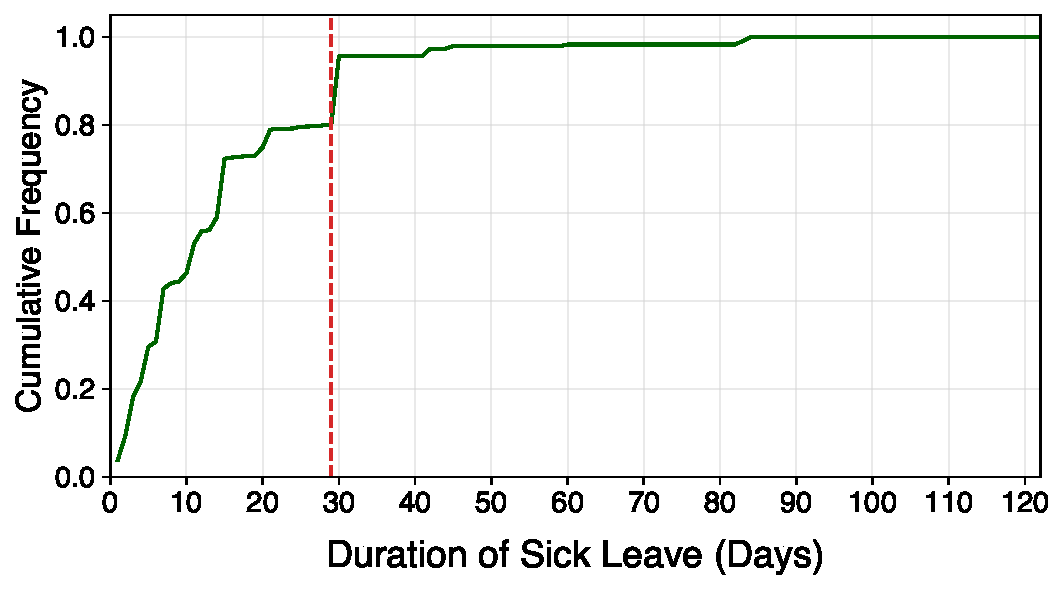
\includegraphics[width=0.70\linewidth]{cdf.pdf}
    \captionsetup{justification=centerlast}
    \caption{Empirical Cumulative Distribution of Sick Leave Durations. \\ A red dashed line is placed at 29 days.}
    \label{fig:cdf}
\end{figure}



We first make use of this distinction to set up our physician quality bins. We design a \textit{quality score} variable by physician based on the three following criteria:\footnote{SEE APPENDIX}
\begin{enumerate}[label=\roman*, itemsep=0pt, topsep=0pt]
    \item Average duration of sick leaves issued.
    \item Percentage of sick leaves of 30+ days over total in sampled period.
    \item Amount of sick leaves of 30+ days issued.
\end{enumerate}

The quality bin to which a physician is assigned corresponds to the decile rank of \textit{quality score} to which they belong. SEEEE APPENDIIIIIIX.

This procedure does perhaps amount to an over-exhertion of our data sample, recognizing that by taking qualitative results from our model as a presumed basis we somewhat pre-fit our data to the model even before calibration, but it is by no means an econometrically unsanctioned manouver, as the population moments with which we calibrate our parameters contain, in part, different information to that with which we set up the bins themselves, so that identification is in fact possible. 

It would indeed be best to assign a quality score based on a set of observables wholly separate from those which play the role of endogenous outcomes in our model, but our course of action is sufficient for our purpose, which isn't to \textit{falsify} our framework—built upon observations and findings established in the relevant literature—but to showcase it and present an approach for its estimation.

\subsection{Data Moments}

Our second use of the distinction between overall sick leaves and the `30+ days' subsample is that we use both as data moments to calibrate our parameters. This means we have two moments \textit{per} quality bin, 20 moments in total to fit our model, as we won't consider variation across the $r_j$ / $\tau_j$ axes.

To define both moments formally within our framework, each bin corresponds to a representative physician $j$, where $J = 10$, such that we have two $J$-dimensional vectors, $X$ and $X^{30}$, where the $j$th component of each corresponds respectively to the two following moments for representative physician $j$:
\begin{align}
    X_j \,=\, &  \int_{\bar{\kappa_j}}^{\infty} \int_{0}^{\infty}s_{ij}(\kappa, \gamma)  \,dG(\gamma) \,dF(\kappa) \tag{\ref{eq:s_X}}
\end{align}
\begin{align}
    X_j^{30} \,=\, & \int_{\bar{\kappa}_{\max}}^{\infty} \int_{0}^{\infty}s_{ij}(\kappa, \gamma)  \,dG(\gamma) \,dF(\kappa)
    \label{eq:X30}
\end{align}

The advantage of using this second defined moment, $X^{30}$, lies in its independence from the choice of strategy $\kappa_j$ and its \textit{near} independence from the distribution $G(\gamma)$. Any patient satisfying $\kappa_i > \bar{\kappa}_{\max}$ will, by definition, be granted sick leave by any physician. The implication of this on the probability $s_{ij}$ that such a patient visits any physician $j$ can be seen as follows:
\begin{align*}
    s_{ij} = \frac{\alpha_{ij}}{\sum_{k = 1}^{J} \alpha_{ik}} & =
    \frac{e^{\lambda u_{ij}}}{\sum\limits_{k : \; u_{ik} \geq 0} \hspace{-0.5em} e^{\lambda u_{ik}}} 
    =
    \frac{e^{\lambda \{V_j \kappa_i + \gamma_i - \tau_j \}}}{\sum\limits_{k : \; u_{ik} \geq 0} \hspace{-0.5em} e^{\lambda \{V_k \kappa_i + \gamma_i - \tau_k \}}} \\
    \\ 
   & = \frac{e^{\lambda \{V_j \kappa_i - \tau_j \}} \cancel{e^{\lambda \gamma_i}}}{\sum\limits_{k : \; u_{ik} \geq 0} \hspace{-0.5em} e^{\lambda \{V_k \kappa_i  - \tau_k \}} \cancel{e^{\lambda\gamma_i}}} =
    \frac{e^{\lambda \{V_j \kappa_i - \tau_j \}}}{\sum\limits_{k : \; u_{ik} \geq 0} \hspace{-0.5em} e^{\lambda \{V_k \kappa_i - \tau_k \}}}
\end{align*}

We see that $\gamma_i$ can be factored out of the defining fraction. It still plays a role, however, in the condition of the summation in the denominator. Physicians afforded a strictly positive probability of visit by patient $i$ must meet the $u_{ij} \geq 0$ condition implied by our \textit{free disposal} patient rationality. This in turn requires of one such physician $j$ to fulfill $V_j \kappa_i + \gamma_i \geq \tau_j$. So the scale of $\gamma_i$ still has implications for $X^{30}$ in this regard, only insofar as it may take a physician completely out of rotation for a patient's strategy vector $S_i$. We can see in the Appendix \ref{sec:id} that the moment outcomes of our model fit are 




\newpage

\section{Something}

\vspace{-0.1em}

\begin{figure}[H]
    \centering
    % First subfigure
    \begin{subfigure}[b]{0.46\linewidth}
        \centering
        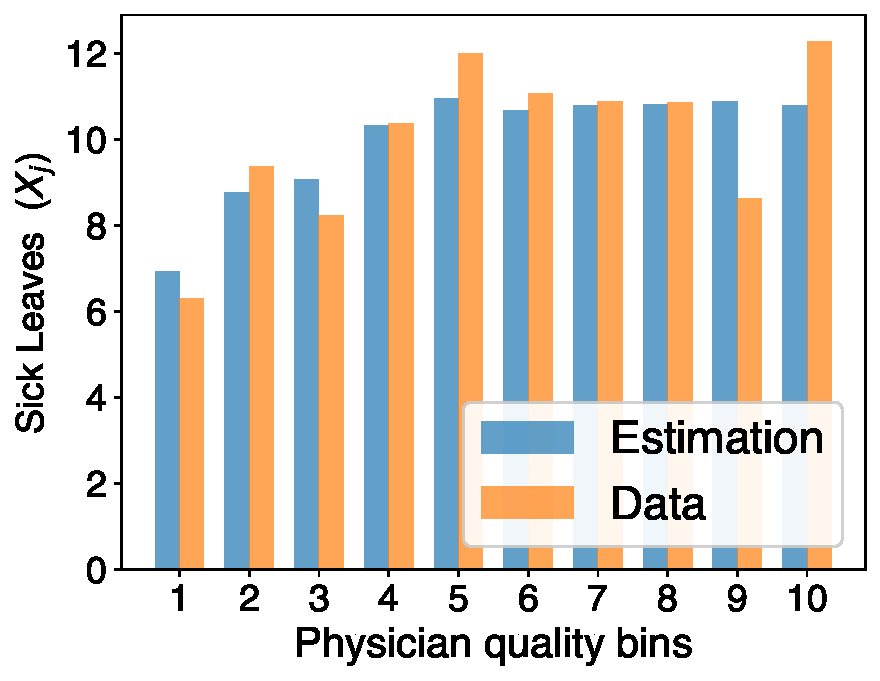
\includegraphics[width=\linewidth]{result_x.pdf}
        
        \caption{$X_j$}

    \end{subfigure}
    \hspace{0.05\linewidth}  % Space between the subfigures
    % Second subfigure
    \begin{subfigure}[b]{0.46\linewidth}
        \centering
        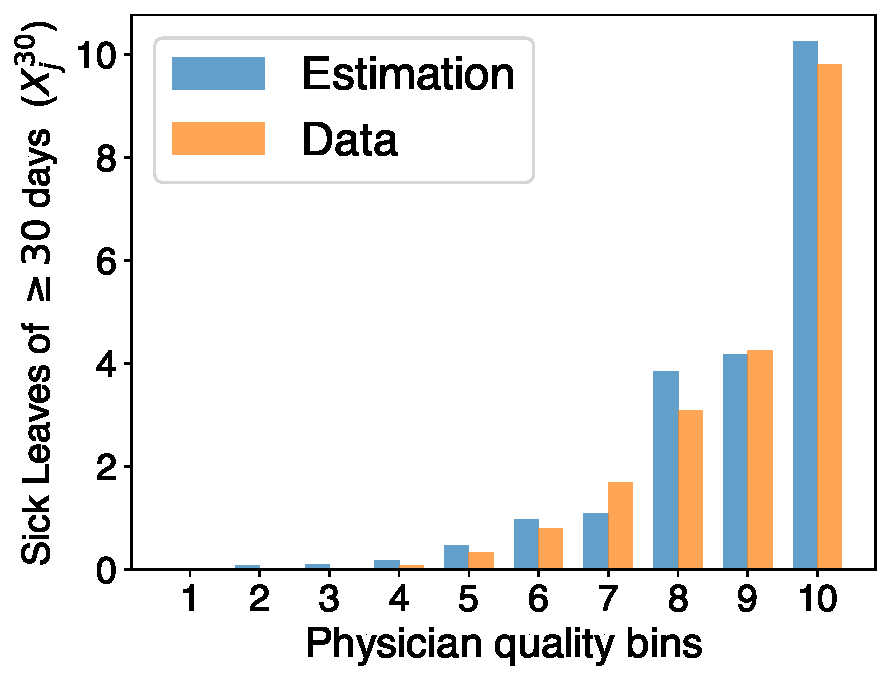
\includegraphics[width=\linewidth]{result_x30.pdf}
        
        \caption{$X_j^{30}$}
    \end{subfigure}


\caption{GMM Results \\ Moments by Quality Bin, Data vs. Model Fit (Estimation)}

\end{figure}

\newpage

\begin{table}[h]
    \centering
    \small
    \begin{tabular}{lcc}
        \toprule
        Parameter  & Value & Source \\
        \midrule
        Physician quality bins && \\
        \hspace{1em}$V_1$ ... $V_{10}$ & $\vec{V}_{1 \times 10}$ & GMM \\
            \\
        Punishment function $P(\cdot)$ && \\
            \hspace{1em}$p$ & 1.953 &  GMM\\
            \\
        Medical need distribution $F(\kappa)$ && \\
            \hspace{1em}$\lambda_F$ & 2 & \hspace{0.25em} Normalization\\
            \\
        Taste distribution $G(\gamma)$ \\
            \hspace{1em}$\mu$ & 73.997 &  GMM\\
            \hspace{1em}$\sigma$ & 18.492 &  GMM\\
            \\
        Maximum threshold level && \\
            \hspace{1em}$\bar{\kappa}_{\max}$ & 0.763 &  GMM\\
            \\
        Logit model parameter && \\
            \hspace{1em}$\lambda_s$ & 0.842 & GMM\\
            \\
        Revenue/cost of visit && \\
            \hspace{1em}$r_j$ & 21.182 & Data \\
            \hspace{1em}$\tau_j$ & 8.944 & Data \\
        \bottomrule 
    \end{tabular}
    \caption{Model parameters}
    \end{table}
    

\end{document}